\chapter{Metod}

\section{Observationer}
Observationer genomfördes med radioteleskop vid Albanova under två separata tillfällen, kvällen 2018-09-19 och förmiddagen 2018-09-29. Teleskopet riktades successivt mot longituder med $5\degree$ mellanrum mellan $0\degree$ och $190\degree$ utefter det galaktiska koordinatsystemet. Latituden hölls konstant vid $0\degree$. Alla observationer gjordes under 90s och återfinns i bilaga 1.

Observationerna analyserades i två steg. I det första steget användes programmet xs\footnote{\url{http://satorchi.net/specsoft/specsoft.php}}, som utvecklades av forskare vid Chalmers för användning inom astrofysik, för att räkna ut de observerade molnens hastighet gentemot oss. I praktiken angavs gissningar till programmet, där programmet sedan anpassade kurvor till den data som fanns tillgänglig i förhållande till gissningarna. De anpassade kurvorna gav oss en genomsnittlig våglängd för fotoner från varje moln varpå programmet jämförde den förväntade våglängden med den uppmätta och räknade ut molnets relativa hastighet gentemot jorden samt storleken på en standardavvikelse. Vi noterade också den högsta uppmätta hastigheten $v_{\mathrm{max}}$ (se figur \ref{fig:multiple_clouds}b).

\begin{figure}
    \centering
    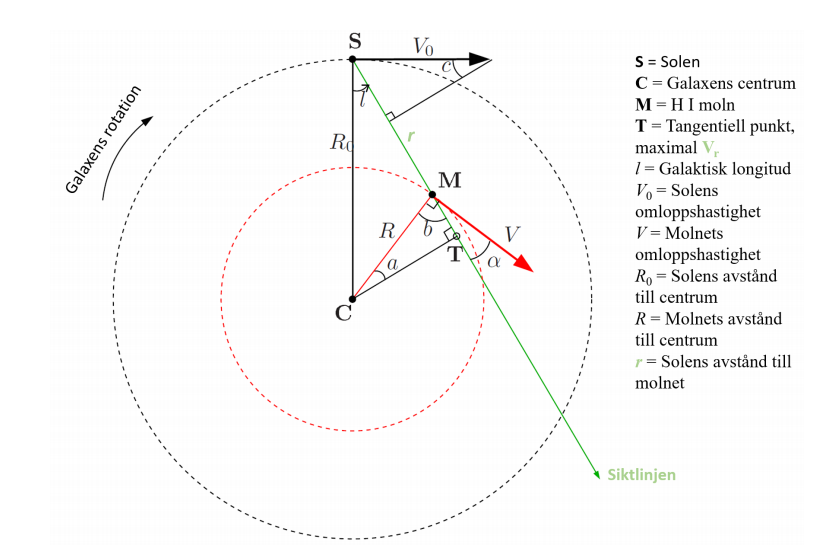
\includegraphics[width=\textwidth]{pics/trigonometri.png}
    \caption{Vintergatan ur ett trigonometriskt perspektiv.}
    \label{fig:trig}
\end{figure}

\section{Trigonometri}

Se figur \ref{fig:trig} för en schematisk ritning över Vintergatan ur ett trigonometriskt perspektiv.

För varje mätning vid en viss longitud $l$ antogs $v_{\mathrm{max}}$ (den maximalt uppmätta hastigheten) vara hastigheten i punkten $T$. Detta eftersom molnets hastighetsvektor $V$ går parallellt med siktlinjen.
För vätet i punkten $T$ antogs
\begin{equation*}
V = V_{\mathrm{max}} + V_{\mathrm{sol}} = V_{\mathrm{max}} + V_0 \cdot \mathrm{sin}(l),
\end{equation*}

där $V_0$ beskriver solens rotationshastighet kring galaxen och $V_{\mathrm{sol}}$ beskriver solens hastighet längs med siktlinjen, samt

\begin{equation*}
    \mathrm{sin}(l) = \frac{R}{R_0} \Rightarrow R = R_0 \cdot \mathrm{sin}(l).
\end{equation*}

Molnets hastighet relativt mot jorden ($V_R$) i punkten T sattes till $V \cdot \mathrm{cos}(\alpha) - V_0 \cdot \mathrm{sin}(c)$. $V \cdot \mathrm{cos}(\alpha)$ beskriver molnets hastighetskomposant i siktlinjen och $V_0 \cdot \mathrm{sin}(c)$ beskriver solens hastighetskomposant i siktlinjen.  Följande antogs:
\begin{gather*}
    90\degree - l = 180\degree - 90\degree - c \Rightarrow l = c \\
    \alpha = 90\degree - b \Rightarrow \mathrm{cos}(\alpha) = \mathrm{cos}(90\degree - b) = \mathrm{sin}(b) \\
    \lvert \mathrm{CT} \rvert = R \cdot \mathrm{sin}(b) = R_0 \cdot \mathrm{sin}(l) \Rightarrow \mathrm{sin}(b) = \frac{R_0}{R} \cdot \mathrm{sin}(l) \ (= \mathrm{cos}(\alpha))\\
\end{gather*}
Värdena på $\mathrm{cos}(\alpha)$ och $c$ sattes in för att lösa $V_R$.

\begin{equation*}
    V_R = V \cdot \mathrm{cos}(\alpha) - V_0 \cdot \mathrm{sin}(c) = V \cdot \frac{R_0}{R} \cdot \mathrm{sin}(l) - V_0 \cdot \mathrm{sin}(l)
\end{equation*}

Utifrån figur \ref{fig:rotation_our} som ritades upp antogs att rotationshastigheten V för allt väte, även det utanför punkten T, var konstant och lika stort som solens rotationshastighet $V_0$, ungefär 220 km/s.

\begin{figure}
    \centering
    \begin{tikzpicture}
        \begin{axis} [
            ylabel=$V_R$ (km/s), ylabel near ticks,
            xlabel=$R$ (kpc), xlabel near ticks,
            xticklabels={1,2,3,4,5,6,7,8,9},
            scale=0.75,
            label style={font=\small}
        ]
            \addplot [mark=*, smooth] table [col sep=comma] {Book1.csv};
        \end{axis}
    \end{tikzpicture}  
    \caption{$V_R$ med avseende på $R$ i punkten T för mätningar $0\degree \leq l \leq 90\degree.$}
    \label{fig:rotation_our}
\end{figure}

    %R = \frac{V_0 \cdot R_0 \cdot \mathrm{sin}(l)}{V_R + V_0 \cdot \mathrm{sin}(l)}


Cosinussatsen gav $R^2 = R_0^2 \cdot r \cdot \mathrm{cos}(l)$ och PQ-formeln gav \\$r = R_0 \cdot \mathrm{cos}(l) \pm \sqrt{R^2-R_0^2 \cdot \mathrm{sin}^2(l)}$.

För att konstruera en vetenskapligt acceptabel karta av dessa värden beaktades den felmariginal som undersökningen påverkades av. Vid användningen av dessa felmariginaler togs det hänsyn till till det faktum att de värden som led av felmarignalen gav upphov till nya värden; felen fortplantades därför genom hela undersökningen. Därför användes formlerna \ref{eq:eR} och \ref{eq:er}\autocite{wiki:fel} där $e_x$ defineras som felmarginalen för x. Felmarginalen för konstanterna $V_0$ och $R_0$ bortsågs då dessa värden är bestämda med mycket högre säkerhet än våra mätvärden.

\begin{equation} \label{eq:eR}
    \lvert e_R \rvert \leq \lvert \frac{R_0 \cdot V_0}{(V_R + V_0)^2} \rvert \cdot \lvert e_{V_r} \rvert
\end{equation}

\begin{equation} \label{eq:er}
    \lvert e_r \rvert \leq \lvert \frac{R}{\sqrt{R^2 - R_0^2 \cdot \mathrm{sin}^2(l)}} \rvert \cdot \lvert e_R \rvert
\end{equation}

%[2] förklara skillnaden mellan v_sol och v_0